\section{Generalized Additive Model}
In this section, we explore one of the most intuitive methods of fitting a binary-response data set. General additive models (GAM) are a natural extension of generalized linear models (GLM), which accept response(s) distributed as a member of the exponential family through the use of link function, by allowing covariates to be modeled with both parametric specifications and nonparametric techniques. Predictors \texttt{degree}, \texttt{decision\_method}, \texttt{decision\_month}, \texttt{gre}, \texttt{status}, \texttt{uni\_faclty} and \texttt{uni\_pub} are used in this section. A derived variable, \texttt{gpa}, is constructed by addition of \texttt{gre\_quant}, \texttt{gre\_verbal} and \texttt{gre\_writing}, based on the assumption that final decisions made may be related to the overall score only.
\subsection{Logistic Regression}
To start with, we consider a canonical logistic regression, whose performance, evaluated by area under the receiver operating characteristic curve (AUC), will be regarded as a benchmark for the project. The value of AUC ranges from 0 to 1, depending on the discriminating power of each model. A larger AUC value indicates better separation of the data, while a value equal to 0.5 implies the model does no better than simply tossing a coin.
\par Parameterization of a good-old logistic regression model is specified below.
\begin{align}
\log\left(\frac{p}{1-p}\right)=\mathbf{x}^\top\boldsymbol{\beta}+\beta_0
\end{align}
where $p=P(Y=1)$ is the probability of the candidate being accepted by the school, and $\mathbf{x}$ is a vector of predictors, which can be either numerical and categorical. 
\par Forward selection is a greedy approach of variable selection by including one independent variable which helps explain the most deviance. This procedure, based on Alkaike's Information Criteria (AIC), measures goodness-of-fit using a penalized maximum likelihood, imposing greater penalty on models with higher complexity. The result suggests a model including all predictors (AIC=5574.28).
\par One may also be interested in whether the two types of degrees have different requirements or selection criteria for candidates with the same academic merits and/or applying under the same category. Based on this motivation, three interaction effects (\texttt{degree:status}, \texttt{degree:gpa} and \texttt{degree:gre}) are consequently added to the model fitted above. However, only \texttt{degree:status} has a significant effect under 5\% level of significance. The inclusion of such effect can be further supported by the AIC statistic, which is brought down to 5570.2. The AUC on test data set is evaluated as 0.716.

\subsection{The Lasso}
Now we approach the variable selection problem again with another popular method, the lasso, which is a shrinkage method of the regression coefficients by putting a constraint on the $L_1$-norm of $\boldsymbol{\beta}$. The parameter estimate can be written as the solution to an optimization problem.
\begin{align}
\widehat{\boldsymbol{\beta}}^{\text{lasso}}=\underset{\boldsymbol{\beta}}{\arg\min}\left\{\sum_i\left[\log\left(\frac{p_i}{1-p_i}\right)-\mathbf{x}^\top\boldsymbol{\beta}-\beta_0\right]^2+\lambda\|\boldsymbol{\beta}\|_1\right\}
\end{align}
where $\lambda$ controls the extent to which the regression coefficients are suppressed. In particular, the lasso, as opposed to ridge regression with penalty laid on the $L_2$-norm, has a variable selection power.

\begin{figure}[htpb]
  \centering
  \def\svgwidth{0.8\textwidth}
  % Created by tikzDevice version 0.11 on 2018-04-28 09:20:55
% !TEX encoding = UTF-8 Unicode
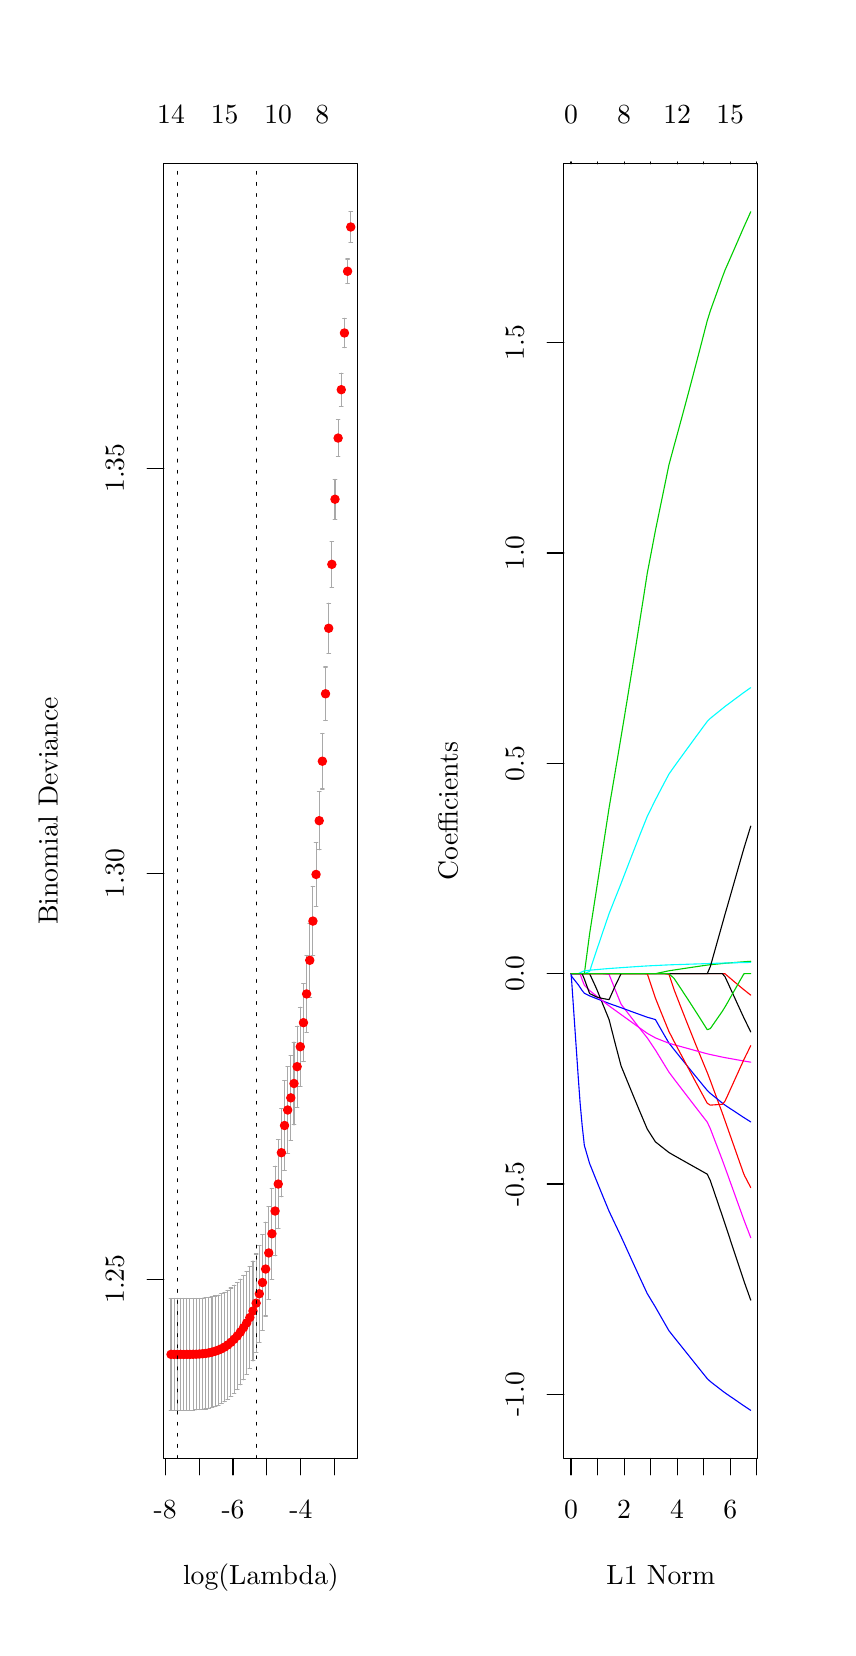
\begin{tikzpicture}[x=1pt,y=1pt]
\definecolor{fillColor}{RGB}{255,255,255}
\path[use as bounding box,fill=fillColor,fill opacity=0.00] (0,0) rectangle (289.08,578.16);
\begin{scope}
\path[clip] (  0.00,  0.00) rectangle (289.08,578.16);
\definecolor{drawColor}{RGB}{0,0,0}

\path[draw=drawColor,line width= 0.4pt,line join=round,line cap=round] ( 49.71, 61.20) -- (110.95, 61.20);

\path[draw=drawColor,line width= 0.4pt,line join=round,line cap=round] ( 49.71, 61.20) -- ( 49.71, 55.20);

\path[draw=drawColor,line width= 0.4pt,line join=round,line cap=round] ( 61.96, 61.20) -- ( 61.96, 55.20);

\path[draw=drawColor,line width= 0.4pt,line join=round,line cap=round] ( 74.21, 61.20) -- ( 74.21, 55.20);

\path[draw=drawColor,line width= 0.4pt,line join=round,line cap=round] ( 86.45, 61.20) -- ( 86.45, 55.20);

\path[draw=drawColor,line width= 0.4pt,line join=round,line cap=round] ( 98.70, 61.20) -- ( 98.70, 55.20);

\path[draw=drawColor,line width= 0.4pt,line join=round,line cap=round] (110.95, 61.20) -- (110.95, 55.20);

\node[text=drawColor,anchor=base,inner sep=0pt, outer sep=0pt, scale=  1.00] at ( 49.71, 39.60) {-8};

\node[text=drawColor,anchor=base,inner sep=0pt, outer sep=0pt, scale=  1.00] at ( 74.21, 39.60) {-6};

\node[text=drawColor,anchor=base,inner sep=0pt, outer sep=0pt, scale=  1.00] at ( 98.70, 39.60) {-4};

\path[draw=drawColor,line width= 0.4pt,line join=round,line cap=round] ( 49.20,125.93) -- ( 49.20,419.01);

\path[draw=drawColor,line width= 0.4pt,line join=round,line cap=round] ( 49.20,125.93) -- ( 43.20,125.93);

\path[draw=drawColor,line width= 0.4pt,line join=round,line cap=round] ( 49.20,272.47) -- ( 43.20,272.47);

\path[draw=drawColor,line width= 0.4pt,line join=round,line cap=round] ( 49.20,419.01) -- ( 43.20,419.01);

\node[text=drawColor,rotate= 90.00,anchor=base,inner sep=0pt, outer sep=0pt, scale=  1.00] at ( 34.80,125.93) {1.25};

\node[text=drawColor,rotate= 90.00,anchor=base,inner sep=0pt, outer sep=0pt, scale=  1.00] at ( 34.80,272.47) {1.30};

\node[text=drawColor,rotate= 90.00,anchor=base,inner sep=0pt, outer sep=0pt, scale=  1.00] at ( 34.80,419.01) {1.35};

\path[draw=drawColor,line width= 0.4pt,line join=round,line cap=round] ( 49.20, 61.20) --
	(119.34, 61.20) --
	(119.34,528.96) --
	( 49.20,528.96) --
	( 49.20, 61.20);
\end{scope}
\begin{scope}
\path[clip] (  0.00,  0.00) rectangle (144.54,578.16);
\definecolor{drawColor}{RGB}{0,0,0}

\node[text=drawColor,anchor=base,inner sep=0pt, outer sep=0pt, scale=  1.00] at ( 84.27, 15.60) {log(Lambda)};

\node[text=drawColor,rotate= 90.00,anchor=base,inner sep=0pt, outer sep=0pt, scale=  1.00] at ( 10.80,295.08) {Binomial Deviance};
\end{scope}
\begin{scope}
\path[clip] ( 49.20, 61.20) rectangle (119.34,528.96);
\definecolor{drawColor}{RGB}{169,169,169}

\path[draw=drawColor,line width= 0.4pt,line join=round,line cap=round] (116.74,511.64) -- (116.74,500.63);

\path[draw=drawColor,line width= 0.4pt,line join=round,line cap=round] (115.60,494.57) -- (115.60,485.69);

\path[draw=drawColor,line width= 0.4pt,line join=round,line cap=round] (114.46,473.14) -- (114.46,462.51);

\path[draw=drawColor,line width= 0.4pt,line join=round,line cap=round] (113.32,453.33) -- (113.32,441.34);

\path[draw=drawColor,line width= 0.4pt,line join=round,line cap=round] (112.18,436.50) -- (112.18,423.23);

\path[draw=drawColor,line width= 0.4pt,line join=round,line cap=round] (111.05,414.94) -- (111.05,400.57);

\path[draw=drawColor,line width= 0.4pt,line join=round,line cap=round] (109.91,392.45) -- (109.91,376.01);

\path[draw=drawColor,line width= 0.4pt,line join=round,line cap=round] (108.77,370.19) -- (108.77,352.07);

\path[draw=drawColor,line width= 0.4pt,line join=round,line cap=round] (107.63,347.13) -- (107.63,327.78);

\path[draw=drawColor,line width= 0.4pt,line join=round,line cap=round] (106.49,323.13) -- (106.49,303.05);

\path[draw=drawColor,line width= 0.4pt,line join=round,line cap=round] (105.35,302.12) -- (105.35,281.07);

\path[draw=drawColor,line width= 0.4pt,line join=round,line cap=round] (104.21,283.72) -- (104.21,260.63);

\path[draw=drawColor,line width= 0.4pt,line join=round,line cap=round] (103.07,267.84) -- (103.07,242.80);

\path[draw=drawColor,line width= 0.4pt,line join=round,line cap=round] (101.93,254.52) -- (101.93,227.78);

\path[draw=drawColor,line width= 0.4pt,line join=round,line cap=round] (100.79,242.83) -- (100.79,215.18);

\path[draw=drawColor,line width= 0.4pt,line join=round,line cap=round] ( 99.65,232.62) -- ( 99.65,204.60);

\path[draw=drawColor,line width= 0.4pt,line join=round,line cap=round] ( 98.51,224.22) -- ( 98.51,195.64);

\path[draw=drawColor,line width= 0.4pt,line join=round,line cap=round] ( 97.37,217.36) -- ( 97.37,188.08);

\path[draw=drawColor,line width= 0.4pt,line join=round,line cap=round] ( 96.23,211.60) -- ( 96.23,181.66);

\path[draw=drawColor,line width= 0.4pt,line join=round,line cap=round] ( 95.09,206.76) -- ( 95.09,176.15);

\path[draw=drawColor,line width= 0.4pt,line join=round,line cap=round] ( 93.95,202.69) -- ( 93.95,171.44);

\path[draw=drawColor,line width= 0.4pt,line join=round,line cap=round] ( 92.82,197.62) -- ( 92.82,165.27);

\path[draw=drawColor,line width= 0.4pt,line join=round,line cap=round] ( 91.68,187.57) -- ( 91.68,155.68);

\path[draw=drawColor,line width= 0.4pt,line join=round,line cap=round] ( 90.54,176.35) -- ( 90.54,144.25);

\path[draw=drawColor,line width= 0.4pt,line join=round,line cap=round] ( 89.40,166.77) -- ( 89.40,134.33);

\path[draw=drawColor,line width= 0.4pt,line join=round,line cap=round] ( 88.26,158.76) -- ( 88.26,125.92);

\path[draw=drawColor,line width= 0.4pt,line join=round,line cap=round] ( 87.12,152.10) -- ( 87.12,118.73);

\path[draw=drawColor,line width= 0.4pt,line join=round,line cap=round] ( 85.98,146.55) -- ( 85.98,112.64);

\path[draw=drawColor,line width= 0.4pt,line join=round,line cap=round] ( 84.84,141.96) -- ( 84.84,107.49);

\path[draw=drawColor,line width= 0.4pt,line join=round,line cap=round] ( 83.70,138.16) -- ( 83.70,103.15);

\path[draw=drawColor,line width= 0.4pt,line join=round,line cap=round] ( 82.56,135.03) -- ( 82.56, 99.50);

\path[draw=drawColor,line width= 0.4pt,line join=round,line cap=round] ( 81.42,132.45) -- ( 81.42, 96.39);

\path[draw=drawColor,line width= 0.4pt,line join=round,line cap=round] ( 80.28,130.35) -- ( 80.28, 93.77);

\path[draw=drawColor,line width= 0.4pt,line join=round,line cap=round] ( 79.14,128.67) -- ( 79.14, 91.56);

\path[draw=drawColor,line width= 0.4pt,line join=round,line cap=round] ( 78.00,127.24) -- ( 78.00, 89.58);

\path[draw=drawColor,line width= 0.4pt,line join=round,line cap=round] ( 76.86,125.90) -- ( 76.86, 87.74);

\path[draw=drawColor,line width= 0.4pt,line join=round,line cap=round] ( 75.72,124.72) -- ( 75.72, 86.06);

\path[draw=drawColor,line width= 0.4pt,line join=round,line cap=round] ( 74.59,123.77) -- ( 74.59, 84.67);

\path[draw=drawColor,line width= 0.4pt,line join=round,line cap=round] ( 73.45,122.74) -- ( 73.45, 83.48);

\path[draw=drawColor,line width= 0.4pt,line join=round,line cap=round] ( 72.31,121.88) -- ( 72.31, 82.46);

\path[draw=drawColor,line width= 0.4pt,line join=round,line cap=round] ( 71.17,121.17) -- ( 71.17, 81.62);

\path[draw=drawColor,line width= 0.4pt,line join=round,line cap=round] ( 70.03,120.63) -- ( 70.03, 80.95);

\path[draw=drawColor,line width= 0.4pt,line join=round,line cap=round] ( 68.89,120.19) -- ( 68.89, 80.38);

\path[draw=drawColor,line width= 0.4pt,line join=round,line cap=round] ( 67.75,119.85) -- ( 67.75, 79.92);

\path[draw=drawColor,line width= 0.4pt,line join=round,line cap=round] ( 66.61,119.58) -- ( 66.61, 79.55);

\path[draw=drawColor,line width= 0.4pt,line join=round,line cap=round] ( 65.47,119.36) -- ( 65.47, 79.25);

\path[draw=drawColor,line width= 0.4pt,line join=round,line cap=round] ( 64.33,119.18) -- ( 64.33, 79.03);

\path[draw=drawColor,line width= 0.4pt,line join=round,line cap=round] ( 63.19,119.07) -- ( 63.19, 78.88);

\path[draw=drawColor,line width= 0.4pt,line join=round,line cap=round] ( 62.05,118.99) -- ( 62.05, 78.77);

\path[draw=drawColor,line width= 0.4pt,line join=round,line cap=round] ( 60.91,118.95) -- ( 60.91, 78.69);

\path[draw=drawColor,line width= 0.4pt,line join=round,line cap=round] ( 59.77,118.93) -- ( 59.77, 78.63);

\path[draw=drawColor,line width= 0.4pt,line join=round,line cap=round] ( 58.63,118.92) -- ( 58.63, 78.59);

\path[draw=drawColor,line width= 0.4pt,line join=round,line cap=round] ( 57.49,118.93) -- ( 57.49, 78.57);

\path[draw=drawColor,line width= 0.4pt,line join=round,line cap=round] ( 56.36,118.94) -- ( 56.36, 78.55);

\path[draw=drawColor,line width= 0.4pt,line join=round,line cap=round] ( 55.22,118.95) -- ( 55.22, 78.54);

\path[draw=drawColor,line width= 0.4pt,line join=round,line cap=round] ( 54.08,118.96) -- ( 54.08, 78.53);

\path[draw=drawColor,line width= 0.4pt,line join=round,line cap=round] ( 52.94,118.97) -- ( 52.94, 78.53);

\path[draw=drawColor,line width= 0.4pt,line join=round,line cap=round] ( 51.80,118.99) -- ( 51.80, 78.52);

\path[draw=drawColor,line width= 0.4pt,line join=round,line cap=round] (116.09,511.64) -- (117.39,511.64);

\path[draw=drawColor,line width= 0.4pt,line join=round,line cap=round] (114.95,494.57) -- (116.25,494.57);

\path[draw=drawColor,line width= 0.4pt,line join=round,line cap=round] (113.81,473.14) -- (115.11,473.14);

\path[draw=drawColor,line width= 0.4pt,line join=round,line cap=round] (112.67,453.33) -- (113.97,453.33);

\path[draw=drawColor,line width= 0.4pt,line join=round,line cap=round] (111.54,436.50) -- (112.83,436.50);

\path[draw=drawColor,line width= 0.4pt,line join=round,line cap=round] (110.40,414.94) -- (111.69,414.94);

\path[draw=drawColor,line width= 0.4pt,line join=round,line cap=round] (109.26,392.45) -- (110.56,392.45);

\path[draw=drawColor,line width= 0.4pt,line join=round,line cap=round] (108.12,370.19) -- (109.42,370.19);

\path[draw=drawColor,line width= 0.4pt,line join=round,line cap=round] (106.98,347.13) -- (108.28,347.13);

\path[draw=drawColor,line width= 0.4pt,line join=round,line cap=round] (105.84,323.13) -- (107.14,323.13);

\path[draw=drawColor,line width= 0.4pt,line join=round,line cap=round] (104.70,302.12) -- (106.00,302.12);

\path[draw=drawColor,line width= 0.4pt,line join=round,line cap=round] (103.56,283.72) -- (104.86,283.72);

\path[draw=drawColor,line width= 0.4pt,line join=round,line cap=round] (102.42,267.84) -- (103.72,267.84);

\path[draw=drawColor,line width= 0.4pt,line join=round,line cap=round] (101.28,254.52) -- (102.58,254.52);

\path[draw=drawColor,line width= 0.4pt,line join=round,line cap=round] (100.14,242.83) -- (101.44,242.83);

\path[draw=drawColor,line width= 0.4pt,line join=round,line cap=round] ( 99.00,232.62) -- (100.30,232.62);

\path[draw=drawColor,line width= 0.4pt,line join=round,line cap=round] ( 97.86,224.22) -- ( 99.16,224.22);

\path[draw=drawColor,line width= 0.4pt,line join=round,line cap=round] ( 96.72,217.36) -- ( 98.02,217.36);

\path[draw=drawColor,line width= 0.4pt,line join=round,line cap=round] ( 95.58,211.60) -- ( 96.88,211.60);

\path[draw=drawColor,line width= 0.4pt,line join=round,line cap=round] ( 94.44,206.76) -- ( 95.74,206.76);

\path[draw=drawColor,line width= 0.4pt,line join=round,line cap=round] ( 93.31,202.69) -- ( 94.60,202.69);

\path[draw=drawColor,line width= 0.4pt,line join=round,line cap=round] ( 92.17,197.62) -- ( 93.46,197.62);

\path[draw=drawColor,line width= 0.4pt,line join=round,line cap=round] ( 91.03,187.57) -- ( 92.33,187.57);

\path[draw=drawColor,line width= 0.4pt,line join=round,line cap=round] ( 89.89,176.35) -- ( 91.19,176.35);

\path[draw=drawColor,line width= 0.4pt,line join=round,line cap=round] ( 88.75,166.77) -- ( 90.05,166.77);

\path[draw=drawColor,line width= 0.4pt,line join=round,line cap=round] ( 87.61,158.76) -- ( 88.91,158.76);

\path[draw=drawColor,line width= 0.4pt,line join=round,line cap=round] ( 86.47,152.10) -- ( 87.77,152.10);

\path[draw=drawColor,line width= 0.4pt,line join=round,line cap=round] ( 85.33,146.55) -- ( 86.63,146.55);

\path[draw=drawColor,line width= 0.4pt,line join=round,line cap=round] ( 84.19,141.96) -- ( 85.49,141.96);

\path[draw=drawColor,line width= 0.4pt,line join=round,line cap=round] ( 83.05,138.16) -- ( 84.35,138.16);

\path[draw=drawColor,line width= 0.4pt,line join=round,line cap=round] ( 81.91,135.03) -- ( 83.21,135.03);

\path[draw=drawColor,line width= 0.4pt,line join=round,line cap=round] ( 80.77,132.45) -- ( 82.07,132.45);

\path[draw=drawColor,line width= 0.4pt,line join=round,line cap=round] ( 79.63,130.35) -- ( 80.93,130.35);

\path[draw=drawColor,line width= 0.4pt,line join=round,line cap=round] ( 78.49,128.67) -- ( 79.79,128.67);

\path[draw=drawColor,line width= 0.4pt,line join=round,line cap=round] ( 77.35,127.24) -- ( 78.65,127.24);

\path[draw=drawColor,line width= 0.4pt,line join=round,line cap=round] ( 76.21,125.90) -- ( 77.51,125.90);

\path[draw=drawColor,line width= 0.4pt,line join=round,line cap=round] ( 75.08,124.72) -- ( 76.37,124.72);

\path[draw=drawColor,line width= 0.4pt,line join=round,line cap=round] ( 73.94,123.77) -- ( 75.23,123.77);

\path[draw=drawColor,line width= 0.4pt,line join=round,line cap=round] ( 72.80,122.74) -- ( 74.10,122.74);

\path[draw=drawColor,line width= 0.4pt,line join=round,line cap=round] ( 71.66,121.88) -- ( 72.96,121.88);

\path[draw=drawColor,line width= 0.4pt,line join=round,line cap=round] ( 70.52,121.17) -- ( 71.82,121.17);

\path[draw=drawColor,line width= 0.4pt,line join=round,line cap=round] ( 69.38,120.63) -- ( 70.68,120.63);

\path[draw=drawColor,line width= 0.4pt,line join=round,line cap=round] ( 68.24,120.19) -- ( 69.54,120.19);

\path[draw=drawColor,line width= 0.4pt,line join=round,line cap=round] ( 67.10,119.85) -- ( 68.40,119.85);

\path[draw=drawColor,line width= 0.4pt,line join=round,line cap=round] ( 65.96,119.58) -- ( 67.26,119.58);

\path[draw=drawColor,line width= 0.4pt,line join=round,line cap=round] ( 64.82,119.36) -- ( 66.12,119.36);

\path[draw=drawColor,line width= 0.4pt,line join=round,line cap=round] ( 63.68,119.18) -- ( 64.98,119.18);

\path[draw=drawColor,line width= 0.4pt,line join=round,line cap=round] ( 62.54,119.07) -- ( 63.84,119.07);

\path[draw=drawColor,line width= 0.4pt,line join=round,line cap=round] ( 61.40,118.99) -- ( 62.70,118.99);

\path[draw=drawColor,line width= 0.4pt,line join=round,line cap=round] ( 60.26,118.95) -- ( 61.56,118.95);

\path[draw=drawColor,line width= 0.4pt,line join=round,line cap=round] ( 59.12,118.93) -- ( 60.42,118.93);

\path[draw=drawColor,line width= 0.4pt,line join=round,line cap=round] ( 57.98,118.92) -- ( 59.28,118.92);

\path[draw=drawColor,line width= 0.4pt,line join=round,line cap=round] ( 56.85,118.93) -- ( 58.14,118.93);

\path[draw=drawColor,line width= 0.4pt,line join=round,line cap=round] ( 55.71,118.94) -- ( 57.00,118.94);

\path[draw=drawColor,line width= 0.4pt,line join=round,line cap=round] ( 54.57,118.95) -- ( 55.87,118.95);

\path[draw=drawColor,line width= 0.4pt,line join=round,line cap=round] ( 53.43,118.96) -- ( 54.73,118.96);

\path[draw=drawColor,line width= 0.4pt,line join=round,line cap=round] ( 52.29,118.97) -- ( 53.59,118.97);

\path[draw=drawColor,line width= 0.4pt,line join=round,line cap=round] ( 51.15,118.99) -- ( 52.45,118.99);

\path[draw=drawColor,line width= 0.4pt,line join=round,line cap=round] (116.09,500.63) -- (117.39,500.63);

\path[draw=drawColor,line width= 0.4pt,line join=round,line cap=round] (114.95,485.69) -- (116.25,485.69);

\path[draw=drawColor,line width= 0.4pt,line join=round,line cap=round] (113.81,462.51) -- (115.11,462.51);

\path[draw=drawColor,line width= 0.4pt,line join=round,line cap=round] (112.67,441.34) -- (113.97,441.34);

\path[draw=drawColor,line width= 0.4pt,line join=round,line cap=round] (111.54,423.23) -- (112.83,423.23);

\path[draw=drawColor,line width= 0.4pt,line join=round,line cap=round] (110.40,400.57) -- (111.69,400.57);

\path[draw=drawColor,line width= 0.4pt,line join=round,line cap=round] (109.26,376.01) -- (110.56,376.01);

\path[draw=drawColor,line width= 0.4pt,line join=round,line cap=round] (108.12,352.07) -- (109.42,352.07);

\path[draw=drawColor,line width= 0.4pt,line join=round,line cap=round] (106.98,327.78) -- (108.28,327.78);

\path[draw=drawColor,line width= 0.4pt,line join=round,line cap=round] (105.84,303.05) -- (107.14,303.05);

\path[draw=drawColor,line width= 0.4pt,line join=round,line cap=round] (104.70,281.07) -- (106.00,281.07);

\path[draw=drawColor,line width= 0.4pt,line join=round,line cap=round] (103.56,260.63) -- (104.86,260.63);

\path[draw=drawColor,line width= 0.4pt,line join=round,line cap=round] (102.42,242.80) -- (103.72,242.80);

\path[draw=drawColor,line width= 0.4pt,line join=round,line cap=round] (101.28,227.78) -- (102.58,227.78);

\path[draw=drawColor,line width= 0.4pt,line join=round,line cap=round] (100.14,215.18) -- (101.44,215.18);

\path[draw=drawColor,line width= 0.4pt,line join=round,line cap=round] ( 99.00,204.60) -- (100.30,204.60);

\path[draw=drawColor,line width= 0.4pt,line join=round,line cap=round] ( 97.86,195.64) -- ( 99.16,195.64);

\path[draw=drawColor,line width= 0.4pt,line join=round,line cap=round] ( 96.72,188.08) -- ( 98.02,188.08);

\path[draw=drawColor,line width= 0.4pt,line join=round,line cap=round] ( 95.58,181.66) -- ( 96.88,181.66);

\path[draw=drawColor,line width= 0.4pt,line join=round,line cap=round] ( 94.44,176.15) -- ( 95.74,176.15);

\path[draw=drawColor,line width= 0.4pt,line join=round,line cap=round] ( 93.31,171.44) -- ( 94.60,171.44);

\path[draw=drawColor,line width= 0.4pt,line join=round,line cap=round] ( 92.17,165.27) -- ( 93.46,165.27);

\path[draw=drawColor,line width= 0.4pt,line join=round,line cap=round] ( 91.03,155.68) -- ( 92.33,155.68);

\path[draw=drawColor,line width= 0.4pt,line join=round,line cap=round] ( 89.89,144.25) -- ( 91.19,144.25);

\path[draw=drawColor,line width= 0.4pt,line join=round,line cap=round] ( 88.75,134.33) -- ( 90.05,134.33);

\path[draw=drawColor,line width= 0.4pt,line join=round,line cap=round] ( 87.61,125.92) -- ( 88.91,125.92);

\path[draw=drawColor,line width= 0.4pt,line join=round,line cap=round] ( 86.47,118.73) -- ( 87.77,118.73);

\path[draw=drawColor,line width= 0.4pt,line join=round,line cap=round] ( 85.33,112.64) -- ( 86.63,112.64);

\path[draw=drawColor,line width= 0.4pt,line join=round,line cap=round] ( 84.19,107.49) -- ( 85.49,107.49);

\path[draw=drawColor,line width= 0.4pt,line join=round,line cap=round] ( 83.05,103.15) -- ( 84.35,103.15);

\path[draw=drawColor,line width= 0.4pt,line join=round,line cap=round] ( 81.91, 99.50) -- ( 83.21, 99.50);

\path[draw=drawColor,line width= 0.4pt,line join=round,line cap=round] ( 80.77, 96.39) -- ( 82.07, 96.39);

\path[draw=drawColor,line width= 0.4pt,line join=round,line cap=round] ( 79.63, 93.77) -- ( 80.93, 93.77);

\path[draw=drawColor,line width= 0.4pt,line join=round,line cap=round] ( 78.49, 91.56) -- ( 79.79, 91.56);

\path[draw=drawColor,line width= 0.4pt,line join=round,line cap=round] ( 77.35, 89.58) -- ( 78.65, 89.58);

\path[draw=drawColor,line width= 0.4pt,line join=round,line cap=round] ( 76.21, 87.74) -- ( 77.51, 87.74);

\path[draw=drawColor,line width= 0.4pt,line join=round,line cap=round] ( 75.08, 86.06) -- ( 76.37, 86.06);

\path[draw=drawColor,line width= 0.4pt,line join=round,line cap=round] ( 73.94, 84.67) -- ( 75.23, 84.67);

\path[draw=drawColor,line width= 0.4pt,line join=round,line cap=round] ( 72.80, 83.48) -- ( 74.10, 83.48);

\path[draw=drawColor,line width= 0.4pt,line join=round,line cap=round] ( 71.66, 82.46) -- ( 72.96, 82.46);

\path[draw=drawColor,line width= 0.4pt,line join=round,line cap=round] ( 70.52, 81.62) -- ( 71.82, 81.62);

\path[draw=drawColor,line width= 0.4pt,line join=round,line cap=round] ( 69.38, 80.95) -- ( 70.68, 80.95);

\path[draw=drawColor,line width= 0.4pt,line join=round,line cap=round] ( 68.24, 80.38) -- ( 69.54, 80.38);

\path[draw=drawColor,line width= 0.4pt,line join=round,line cap=round] ( 67.10, 79.92) -- ( 68.40, 79.92);

\path[draw=drawColor,line width= 0.4pt,line join=round,line cap=round] ( 65.96, 79.55) -- ( 67.26, 79.55);

\path[draw=drawColor,line width= 0.4pt,line join=round,line cap=round] ( 64.82, 79.25) -- ( 66.12, 79.25);

\path[draw=drawColor,line width= 0.4pt,line join=round,line cap=round] ( 63.68, 79.03) -- ( 64.98, 79.03);

\path[draw=drawColor,line width= 0.4pt,line join=round,line cap=round] ( 62.54, 78.88) -- ( 63.84, 78.88);

\path[draw=drawColor,line width= 0.4pt,line join=round,line cap=round] ( 61.40, 78.77) -- ( 62.70, 78.77);

\path[draw=drawColor,line width= 0.4pt,line join=round,line cap=round] ( 60.26, 78.69) -- ( 61.56, 78.69);

\path[draw=drawColor,line width= 0.4pt,line join=round,line cap=round] ( 59.12, 78.63) -- ( 60.42, 78.63);

\path[draw=drawColor,line width= 0.4pt,line join=round,line cap=round] ( 57.98, 78.59) -- ( 59.28, 78.59);

\path[draw=drawColor,line width= 0.4pt,line join=round,line cap=round] ( 56.85, 78.57) -- ( 58.14, 78.57);

\path[draw=drawColor,line width= 0.4pt,line join=round,line cap=round] ( 55.71, 78.55) -- ( 57.00, 78.55);

\path[draw=drawColor,line width= 0.4pt,line join=round,line cap=round] ( 54.57, 78.54) -- ( 55.87, 78.54);

\path[draw=drawColor,line width= 0.4pt,line join=round,line cap=round] ( 53.43, 78.53) -- ( 54.73, 78.53);

\path[draw=drawColor,line width= 0.4pt,line join=round,line cap=round] ( 52.29, 78.53) -- ( 53.59, 78.53);

\path[draw=drawColor,line width= 0.4pt,line join=round,line cap=round] ( 51.15, 78.52) -- ( 52.45, 78.52);
\definecolor{drawColor}{RGB}{255,0,0}
\definecolor{fillColor}{RGB}{255,0,0}

\path[draw=drawColor,line width= 0.4pt,line join=round,line cap=round,fill=fillColor] (116.74,506.13) circle (  1.50);

\path[draw=drawColor,line width= 0.4pt,line join=round,line cap=round,fill=fillColor] (115.60,490.13) circle (  1.50);

\path[draw=drawColor,line width= 0.4pt,line join=round,line cap=round,fill=fillColor] (114.46,467.83) circle (  1.50);

\path[draw=drawColor,line width= 0.4pt,line join=round,line cap=round,fill=fillColor] (113.32,447.34) circle (  1.50);

\path[draw=drawColor,line width= 0.4pt,line join=round,line cap=round,fill=fillColor] (112.18,429.86) circle (  1.50);

\path[draw=drawColor,line width= 0.4pt,line join=round,line cap=round,fill=fillColor] (111.05,407.76) circle (  1.50);

\path[draw=drawColor,line width= 0.4pt,line join=round,line cap=round,fill=fillColor] (109.91,384.23) circle (  1.50);

\path[draw=drawColor,line width= 0.4pt,line join=round,line cap=round,fill=fillColor] (108.77,361.13) circle (  1.50);

\path[draw=drawColor,line width= 0.4pt,line join=round,line cap=round,fill=fillColor] (107.63,337.46) circle (  1.50);

\path[draw=drawColor,line width= 0.4pt,line join=round,line cap=round,fill=fillColor] (106.49,313.09) circle (  1.50);

\path[draw=drawColor,line width= 0.4pt,line join=round,line cap=round,fill=fillColor] (105.35,291.60) circle (  1.50);

\path[draw=drawColor,line width= 0.4pt,line join=round,line cap=round,fill=fillColor] (104.21,272.18) circle (  1.50);

\path[draw=drawColor,line width= 0.4pt,line join=round,line cap=round,fill=fillColor] (103.07,255.32) circle (  1.50);

\path[draw=drawColor,line width= 0.4pt,line join=round,line cap=round,fill=fillColor] (101.93,241.15) circle (  1.50);

\path[draw=drawColor,line width= 0.4pt,line join=round,line cap=round,fill=fillColor] (100.79,229.00) circle (  1.50);

\path[draw=drawColor,line width= 0.4pt,line join=round,line cap=round,fill=fillColor] ( 99.65,218.61) circle (  1.50);

\path[draw=drawColor,line width= 0.4pt,line join=round,line cap=round,fill=fillColor] ( 98.51,209.93) circle (  1.50);

\path[draw=drawColor,line width= 0.4pt,line join=round,line cap=round,fill=fillColor] ( 97.37,202.72) circle (  1.50);

\path[draw=drawColor,line width= 0.4pt,line join=round,line cap=round,fill=fillColor] ( 96.23,196.63) circle (  1.50);

\path[draw=drawColor,line width= 0.4pt,line join=round,line cap=round,fill=fillColor] ( 95.09,191.45) circle (  1.50);

\path[draw=drawColor,line width= 0.4pt,line join=round,line cap=round,fill=fillColor] ( 93.95,187.06) circle (  1.50);

\path[draw=drawColor,line width= 0.4pt,line join=round,line cap=round,fill=fillColor] ( 92.82,181.45) circle (  1.50);

\path[draw=drawColor,line width= 0.4pt,line join=round,line cap=round,fill=fillColor] ( 91.68,171.63) circle (  1.50);

\path[draw=drawColor,line width= 0.4pt,line join=round,line cap=round,fill=fillColor] ( 90.54,160.30) circle (  1.50);

\path[draw=drawColor,line width= 0.4pt,line join=round,line cap=round,fill=fillColor] ( 89.40,150.55) circle (  1.50);

\path[draw=drawColor,line width= 0.4pt,line join=round,line cap=round,fill=fillColor] ( 88.26,142.34) circle (  1.50);

\path[draw=drawColor,line width= 0.4pt,line join=round,line cap=round,fill=fillColor] ( 87.12,135.41) circle (  1.50);

\path[draw=drawColor,line width= 0.4pt,line join=round,line cap=round,fill=fillColor] ( 85.98,129.59) circle (  1.50);

\path[draw=drawColor,line width= 0.4pt,line join=round,line cap=round,fill=fillColor] ( 84.84,124.72) circle (  1.50);

\path[draw=drawColor,line width= 0.4pt,line join=round,line cap=round,fill=fillColor] ( 83.70,120.66) circle (  1.50);

\path[draw=drawColor,line width= 0.4pt,line join=round,line cap=round,fill=fillColor] ( 82.56,117.26) circle (  1.50);

\path[draw=drawColor,line width= 0.4pt,line join=round,line cap=round,fill=fillColor] ( 81.42,114.42) circle (  1.50);

\path[draw=drawColor,line width= 0.4pt,line join=round,line cap=round,fill=fillColor] ( 80.28,112.06) circle (  1.50);

\path[draw=drawColor,line width= 0.4pt,line join=round,line cap=round,fill=fillColor] ( 79.14,110.11) circle (  1.50);

\path[draw=drawColor,line width= 0.4pt,line join=round,line cap=round,fill=fillColor] ( 78.00,108.41) circle (  1.50);

\path[draw=drawColor,line width= 0.4pt,line join=round,line cap=round,fill=fillColor] ( 76.86,106.82) circle (  1.50);

\path[draw=drawColor,line width= 0.4pt,line join=round,line cap=round,fill=fillColor] ( 75.72,105.39) circle (  1.50);

\path[draw=drawColor,line width= 0.4pt,line join=round,line cap=round,fill=fillColor] ( 74.59,104.22) circle (  1.50);

\path[draw=drawColor,line width= 0.4pt,line join=round,line cap=round,fill=fillColor] ( 73.45,103.11) circle (  1.50);

\path[draw=drawColor,line width= 0.4pt,line join=round,line cap=round,fill=fillColor] ( 72.31,102.17) circle (  1.50);

\path[draw=drawColor,line width= 0.4pt,line join=round,line cap=round,fill=fillColor] ( 71.17,101.40) circle (  1.50);

\path[draw=drawColor,line width= 0.4pt,line join=round,line cap=round,fill=fillColor] ( 70.03,100.79) circle (  1.50);

\path[draw=drawColor,line width= 0.4pt,line join=round,line cap=round,fill=fillColor] ( 68.89,100.29) circle (  1.50);

\path[draw=drawColor,line width= 0.4pt,line join=round,line cap=round,fill=fillColor] ( 67.75, 99.88) circle (  1.50);

\path[draw=drawColor,line width= 0.4pt,line join=round,line cap=round,fill=fillColor] ( 66.61, 99.56) circle (  1.50);

\path[draw=drawColor,line width= 0.4pt,line join=round,line cap=round,fill=fillColor] ( 65.47, 99.30) circle (  1.50);

\path[draw=drawColor,line width= 0.4pt,line join=round,line cap=round,fill=fillColor] ( 64.33, 99.10) circle (  1.50);

\path[draw=drawColor,line width= 0.4pt,line join=round,line cap=round,fill=fillColor] ( 63.19, 98.98) circle (  1.50);

\path[draw=drawColor,line width= 0.4pt,line join=round,line cap=round,fill=fillColor] ( 62.05, 98.88) circle (  1.50);

\path[draw=drawColor,line width= 0.4pt,line join=round,line cap=round,fill=fillColor] ( 60.91, 98.82) circle (  1.50);

\path[draw=drawColor,line width= 0.4pt,line join=round,line cap=round,fill=fillColor] ( 59.77, 98.78) circle (  1.50);

\path[draw=drawColor,line width= 0.4pt,line join=round,line cap=round,fill=fillColor] ( 58.63, 98.75) circle (  1.50);

\path[draw=drawColor,line width= 0.4pt,line join=round,line cap=round,fill=fillColor] ( 57.49, 98.75) circle (  1.50);

\path[draw=drawColor,line width= 0.4pt,line join=round,line cap=round,fill=fillColor] ( 56.36, 98.74) circle (  1.50);

\path[draw=drawColor,line width= 0.4pt,line join=round,line cap=round,fill=fillColor] ( 55.22, 98.75) circle (  1.50);

\path[draw=drawColor,line width= 0.4pt,line join=round,line cap=round,fill=fillColor] ( 54.08, 98.74) circle (  1.50);

\path[draw=drawColor,line width= 0.4pt,line join=round,line cap=round,fill=fillColor] ( 52.94, 98.75) circle (  1.50);

\path[draw=drawColor,line width= 0.4pt,line join=round,line cap=round,fill=fillColor] ( 51.80, 98.75) circle (  1.50);
\end{scope}
\begin{scope}
\path[clip] (  0.00,  0.00) rectangle (289.08,578.16);
\definecolor{drawColor}{RGB}{0,0,0}

\node[text=drawColor,anchor=base,inner sep=0pt, outer sep=0pt, scale=  1.00] at ( 51.80,543.36) {14};

\node[text=drawColor,anchor=base,inner sep=0pt, outer sep=0pt, scale=  1.00] at ( 71.17,543.36) {15};

\node[text=drawColor,anchor=base,inner sep=0pt, outer sep=0pt, scale=  1.00] at ( 90.54,543.36) {10};

\node[text=drawColor,anchor=base,inner sep=0pt, outer sep=0pt, scale=  1.00] at (106.49,543.36) {8};
\end{scope}
\begin{scope}
\path[clip] ( 49.20, 61.20) rectangle (119.34,528.96);
\definecolor{drawColor}{RGB}{0,0,0}

\path[draw=drawColor,line width= 0.4pt,dash pattern=on 1pt off 3pt ,line join=round,line cap=round] ( 54.08, 61.20) -- ( 54.08,528.96);

\path[draw=drawColor,line width= 0.4pt,dash pattern=on 1pt off 3pt ,line join=round,line cap=round] ( 82.56, 61.20) -- ( 82.56,528.96);
\end{scope}
\begin{scope}
\path[clip] (193.74, 61.20) rectangle (263.88,528.96);
\definecolor{drawColor}{RGB}{0,0,0}

\path[draw=drawColor,line width= 0.4pt,line join=round,line cap=round] (196.34,236.32) --
	(196.62,236.32) --
	(197.47,236.32) --
	(198.25,236.32) --
	(198.96,236.32) --
	(199.63,236.32) --
	(200.35,236.32) --
	(201.15,236.32) --
	(203.06,236.32) --
	(205.55,230.89) --
	(207.90,225.10) --
	(210.09,219.72) --
	(212.34,210.92) --
	(214.43,202.97) --
	(216.31,198.37) --
	(218.05,194.12) --
	(219.67,190.20) --
	(221.17,186.58) --
	(222.58,183.25) --
	(223.88,180.18) --
	(225.41,177.77) --
	(226.83,175.56) --
	(228.56,174.18) --
	(230.19,172.90) --
	(231.71,171.70) --
	(233.59,170.61) --
	(235.38,169.60) --
	(237.03,168.67) --
	(238.56,167.81) --
	(239.97,167.02) --
	(241.27,166.28) --
	(242.48,165.61) --
	(243.59,164.98) --
	(244.61,164.41) --
	(245.56,163.88) --
	(246.68,161.53) --
	(247.91,157.91) --
	(249.05,154.57) --
	(250.09,151.50) --
	(251.05,148.68) --
	(251.98,145.86) --
	(252.95,142.97) --
	(253.85,140.24) --
	(254.67,137.77) --
	(255.42,135.52) --
	(256.11,133.41) --
	(256.74,131.52) --
	(257.32,129.76) --
	(257.85,128.18) --
	(258.32,126.75) --
	(258.77,125.40) --
	(259.19,124.21) --
	(259.58,123.10) --
	(259.93,122.13) --
	(260.24,121.27) --
	(260.54,120.43) --
	(260.81,119.65) --
	(261.05,118.98) --
	(261.28,118.34);
\end{scope}
\begin{scope}
\path[clip] (  0.00,  0.00) rectangle (289.08,578.16);
\definecolor{drawColor}{RGB}{0,0,0}

\path[draw=drawColor,line width= 0.4pt,line join=round,line cap=round] (196.34, 61.20) -- (263.46, 61.20);

\path[draw=drawColor,line width= 0.4pt,line join=round,line cap=round] (196.34, 61.20) -- (196.34, 55.20);

\path[draw=drawColor,line width= 0.4pt,line join=round,line cap=round] (205.93, 61.20) -- (205.93, 55.20);

\path[draw=drawColor,line width= 0.4pt,line join=round,line cap=round] (215.52, 61.20) -- (215.52, 55.20);

\path[draw=drawColor,line width= 0.4pt,line join=round,line cap=round] (225.11, 61.20) -- (225.11, 55.20);

\path[draw=drawColor,line width= 0.4pt,line join=round,line cap=round] (234.69, 61.20) -- (234.69, 55.20);

\path[draw=drawColor,line width= 0.4pt,line join=round,line cap=round] (244.28, 61.20) -- (244.28, 55.20);

\path[draw=drawColor,line width= 0.4pt,line join=round,line cap=round] (253.87, 61.20) -- (253.87, 55.20);

\path[draw=drawColor,line width= 0.4pt,line join=round,line cap=round] (263.46, 61.20) -- (263.46, 55.20);

\node[text=drawColor,anchor=base,inner sep=0pt, outer sep=0pt, scale=  1.00] at (196.34, 39.60) {0};

\node[text=drawColor,anchor=base,inner sep=0pt, outer sep=0pt, scale=  1.00] at (215.52, 39.60) {2};

\node[text=drawColor,anchor=base,inner sep=0pt, outer sep=0pt, scale=  1.00] at (234.69, 39.60) {4};

\node[text=drawColor,anchor=base,inner sep=0pt, outer sep=0pt, scale=  1.00] at (253.87, 39.60) {6};

\path[draw=drawColor,line width= 0.4pt,line join=round,line cap=round] (193.74, 84.33) -- (193.74,464.31);

\path[draw=drawColor,line width= 0.4pt,line join=round,line cap=round] (193.74, 84.33) -- (187.74, 84.33);

\path[draw=drawColor,line width= 0.4pt,line join=round,line cap=round] (193.74,160.32) -- (187.74,160.32);

\path[draw=drawColor,line width= 0.4pt,line join=round,line cap=round] (193.74,236.32) -- (187.74,236.32);

\path[draw=drawColor,line width= 0.4pt,line join=round,line cap=round] (193.74,312.32) -- (187.74,312.32);

\path[draw=drawColor,line width= 0.4pt,line join=round,line cap=round] (193.74,388.31) -- (187.74,388.31);

\path[draw=drawColor,line width= 0.4pt,line join=round,line cap=round] (193.74,464.31) -- (187.74,464.31);

\node[text=drawColor,rotate= 90.00,anchor=base,inner sep=0pt, outer sep=0pt, scale=  1.00] at (179.34, 84.33) {-1.0};

\node[text=drawColor,rotate= 90.00,anchor=base,inner sep=0pt, outer sep=0pt, scale=  1.00] at (179.34,160.32) {-0.5};

\node[text=drawColor,rotate= 90.00,anchor=base,inner sep=0pt, outer sep=0pt, scale=  1.00] at (179.34,236.32) {0.0};

\node[text=drawColor,rotate= 90.00,anchor=base,inner sep=0pt, outer sep=0pt, scale=  1.00] at (179.34,312.32) {0.5};

\node[text=drawColor,rotate= 90.00,anchor=base,inner sep=0pt, outer sep=0pt, scale=  1.00] at (179.34,388.31) {1.0};

\node[text=drawColor,rotate= 90.00,anchor=base,inner sep=0pt, outer sep=0pt, scale=  1.00] at (179.34,464.31) {1.5};

\path[draw=drawColor,line width= 0.4pt,line join=round,line cap=round] (193.74, 61.20) --
	(263.88, 61.20) --
	(263.88,528.96) --
	(193.74,528.96) --
	(193.74, 61.20);
\end{scope}
\begin{scope}
\path[clip] (144.54,  0.00) rectangle (289.08,578.16);
\definecolor{drawColor}{RGB}{0,0,0}

\node[text=drawColor,anchor=base,inner sep=0pt, outer sep=0pt, scale=  1.00] at (228.81, 15.60) {L1 Norm};

\node[text=drawColor,rotate= 90.00,anchor=base,inner sep=0pt, outer sep=0pt, scale=  1.00] at (155.34,295.08) {Coefficients};
\end{scope}
\begin{scope}
\path[clip] (193.74, 61.20) rectangle (263.88,528.96);
\definecolor{drawColor}{RGB}{255,0,0}

\path[draw=drawColor,line width= 0.4pt,line join=round,line cap=round] (196.34,236.32) --
	(196.62,236.32) --
	(197.47,236.32) --
	(198.25,236.32) --
	(198.96,236.32) --
	(199.63,236.32) --
	(200.35,236.32) --
	(201.15,236.32) --
	(203.06,236.32) --
	(205.55,236.32) --
	(207.90,236.32) --
	(210.09,236.32) --
	(212.34,236.32) --
	(214.43,236.32) --
	(216.31,236.32) --
	(218.05,236.32) --
	(219.67,236.32) --
	(221.17,236.32) --
	(222.58,236.32) --
	(223.88,236.32) --
	(225.41,236.32) --
	(226.83,236.32) --
	(228.56,236.32) --
	(230.19,236.32) --
	(231.71,236.32) --
	(233.59,236.32) --
	(235.38,236.32) --
	(237.03,236.32) --
	(238.56,236.32) --
	(239.97,236.32) --
	(241.27,236.32) --
	(242.48,236.32) --
	(243.59,236.32) --
	(244.61,236.32) --
	(245.56,236.32) --
	(246.68,236.32) --
	(247.91,236.32) --
	(249.05,236.32) --
	(250.09,236.32) --
	(251.05,236.32) --
	(251.98,236.28) --
	(252.95,235.44) --
	(253.85,234.68) --
	(254.67,233.98) --
	(255.42,233.34) --
	(256.11,232.76) --
	(256.74,232.24) --
	(257.32,231.75) --
	(257.85,231.31) --
	(258.32,230.91) --
	(258.77,230.55) --
	(259.19,230.21) --
	(259.58,229.91) --
	(259.93,229.63) --
	(260.24,229.37) --
	(260.54,229.14) --
	(260.81,228.93) --
	(261.05,228.74) --
	(261.28,228.56);
\definecolor{drawColor}{RGB}{0,205,0}

\path[draw=drawColor,line width= 0.4pt,line join=round,line cap=round] (196.34,236.32) --
	(196.62,236.32) --
	(197.47,236.32) --
	(198.25,236.32) --
	(198.96,236.32) --
	(199.63,236.32) --
	(200.35,236.32) --
	(201.15,236.32) --
	(203.06,250.76) --
	(205.55,266.80) --
	(207.90,282.01) --
	(210.09,296.24) --
	(212.34,309.49) --
	(214.43,321.92) --
	(216.31,333.31) --
	(218.05,344.03) --
	(219.67,354.14) --
	(221.17,363.65) --
	(222.58,372.59) --
	(223.88,380.99) --
	(225.41,388.97) --
	(226.83,396.45) --
	(228.56,404.84) --
	(230.19,412.74) --
	(231.71,420.15) --
	(233.59,427.11) --
	(235.38,433.63) --
	(237.03,439.73) --
	(238.56,445.43) --
	(239.97,450.75) --
	(241.27,455.71) --
	(242.48,460.32) --
	(243.59,464.61) --
	(244.61,468.58) --
	(245.56,472.26) --
	(246.68,475.84) --
	(247.91,479.28) --
	(249.05,482.45) --
	(250.09,485.37) --
	(251.05,488.07) --
	(251.98,490.52) --
	(252.95,492.73) --
	(253.85,494.78) --
	(254.67,496.65) --
	(255.42,498.36) --
	(256.11,499.95) --
	(256.74,501.39) --
	(257.32,502.73) --
	(257.85,503.94) --
	(258.32,505.04) --
	(258.77,506.07) --
	(259.19,507.00) --
	(259.58,507.86) --
	(259.93,508.63) --
	(260.24,509.33) --
	(260.54,509.99) --
	(260.81,510.59) --
	(261.05,511.13) --
	(261.28,511.64);
\definecolor{drawColor}{RGB}{0,0,255}

\path[draw=drawColor,line width= 0.4pt,line join=round,line cap=round] (196.34,236.32) --
	(196.62,232.94) --
	(197.47,220.46) --
	(198.25,209.10) --
	(198.96,198.72) --
	(199.63,189.48) --
	(200.35,181.57) --
	(201.15,174.27) --
	(203.06,167.70) --
	(205.55,161.52) --
	(207.90,155.77) --
	(210.09,150.46) --
	(212.34,145.72) --
	(214.43,141.32) --
	(216.31,137.19) --
	(218.05,133.36) --
	(219.67,129.82) --
	(221.17,126.55) --
	(222.58,123.52) --
	(223.88,120.73) --
	(225.41,118.19) --
	(226.83,115.85) --
	(228.56,112.81) --
	(230.19,109.96) --
	(231.71,107.32) --
	(233.59,104.93) --
	(235.38,102.70) --
	(237.03,100.64) --
	(238.56, 98.73) --
	(239.97, 96.97) --
	(241.27, 95.34) --
	(242.48, 93.84) --
	(243.59, 92.45) --
	(244.61, 91.17) --
	(245.56, 90.00) --
	(246.68, 88.94) --
	(247.91, 87.98) --
	(249.05, 87.11) --
	(250.09, 86.30) --
	(251.05, 85.55) --
	(251.98, 84.86) --
	(252.95, 84.19) --
	(253.85, 83.57) --
	(254.67, 83.01) --
	(255.42, 82.50) --
	(256.11, 82.02) --
	(256.74, 81.59) --
	(257.32, 81.19) --
	(257.85, 80.82) --
	(258.32, 80.49) --
	(258.77, 80.19) --
	(259.19, 79.91) --
	(259.58, 79.65) --
	(259.93, 79.42) --
	(260.24, 79.21) --
	(260.54, 79.02) --
	(260.81, 78.84) --
	(261.05, 78.67) --
	(261.28, 78.52);
\definecolor{drawColor}{RGB}{0,255,255}

\path[draw=drawColor,line width= 0.4pt,line join=round,line cap=round] (196.34,236.32) --
	(196.62,236.32) --
	(197.47,236.32) --
	(198.25,236.32) --
	(198.96,236.32) --
	(199.63,236.32) --
	(200.35,236.32) --
	(201.15,236.32) --
	(203.06,237.15) --
	(205.55,244.65) --
	(207.90,251.61) --
	(210.09,258.01) --
	(212.34,263.70) --
	(214.43,268.94) --
	(216.31,273.84) --
	(218.05,278.35) --
	(219.67,282.51) --
	(221.17,286.35) --
	(222.58,289.89) --
	(223.88,293.15) --
	(225.41,296.26) --
	(226.83,299.13) --
	(228.56,302.46) --
	(230.19,305.56) --
	(231.71,308.42) --
	(233.59,311.10) --
	(235.38,313.57) --
	(237.03,315.84) --
	(238.56,317.94) --
	(239.97,319.87) --
	(241.27,321.66) --
	(242.48,323.29) --
	(243.59,324.81) --
	(244.61,326.19) --
	(245.56,327.46) --
	(246.68,328.58) --
	(247.91,329.58) --
	(249.05,330.50) --
	(250.09,331.33) --
	(251.05,332.11) --
	(251.98,332.87) --
	(252.95,333.59) --
	(253.85,334.26) --
	(254.67,334.87) --
	(255.42,335.43) --
	(256.11,335.94) --
	(256.74,336.41) --
	(257.32,336.84) --
	(257.85,337.23) --
	(258.32,337.59) --
	(258.77,337.92) --
	(259.19,338.21) --
	(259.58,338.48) --
	(259.93,338.73) --
	(260.24,338.95) --
	(260.54,339.16) --
	(260.81,339.35) --
	(261.05,339.52) --
	(261.28,339.67);
\definecolor{drawColor}{RGB}{255,0,255}

\path[draw=drawColor,line width= 0.4pt,line join=round,line cap=round] (196.34,236.32) --
	(196.62,236.32) --
	(197.47,236.32) --
	(198.25,236.32) --
	(198.96,236.32) --
	(199.63,236.32) --
	(200.35,236.32) --
	(201.15,236.32) --
	(203.06,236.32) --
	(205.55,236.32) --
	(207.90,236.32) --
	(210.09,236.08) --
	(212.34,230.40) --
	(214.43,225.29) --
	(216.31,222.83) --
	(218.05,220.57) --
	(219.67,218.47) --
	(221.17,216.54) --
	(222.58,214.76) --
	(223.88,213.12) --
	(225.41,210.84) --
	(226.83,208.74) --
	(228.56,205.89) --
	(230.19,203.23) --
	(231.71,200.76) --
	(233.59,198.24) --
	(235.38,195.90) --
	(237.03,193.74) --
	(238.56,191.75) --
	(239.97,189.91) --
	(241.27,188.22) --
	(242.48,186.66) --
	(243.59,185.22) --
	(244.61,183.90) --
	(245.56,182.69) --
	(246.68,180.29) --
	(247.91,177.06) --
	(249.05,174.09) --
	(250.09,171.37) --
	(251.05,168.85) --
	(251.98,166.29) --
	(252.95,163.63) --
	(253.85,161.12) --
	(254.67,158.85) --
	(255.42,156.78) --
	(256.11,154.84) --
	(256.74,153.10) --
	(257.32,151.48) --
	(257.85,150.03) --
	(258.32,148.71) --
	(258.77,147.47) --
	(259.19,146.37) --
	(259.58,145.34) --
	(259.93,144.44) --
	(260.24,143.64) --
	(260.54,142.86) --
	(260.81,142.13) --
	(261.05,141.52) --
	(261.28,140.92);
\definecolor{drawColor}{RGB}{0,0,0}

\path[draw=drawColor,line width= 0.4pt,line join=round,line cap=round] (196.34,236.32) --
	(196.62,236.32) --
	(197.47,236.32) --
	(198.25,236.32) --
	(198.96,236.32) --
	(199.63,236.32) --
	(200.35,236.32) --
	(201.15,236.32) --
	(203.06,236.32) --
	(205.55,236.32) --
	(207.90,236.32) --
	(210.09,236.32) --
	(212.34,236.32) --
	(214.43,236.32) --
	(216.31,236.32) --
	(218.05,236.32) --
	(219.67,236.32) --
	(221.17,236.32) --
	(222.58,236.32) --
	(223.88,236.32) --
	(225.41,236.32) --
	(226.83,236.32) --
	(228.56,236.32) --
	(230.19,236.32) --
	(231.71,236.32) --
	(233.59,236.32) --
	(235.38,236.32) --
	(237.03,236.32) --
	(238.56,236.32) --
	(239.97,236.32) --
	(241.27,236.32) --
	(242.48,236.32) --
	(243.59,236.32) --
	(244.61,236.32) --
	(245.56,236.32) --
	(246.68,236.32) --
	(247.91,236.32) --
	(249.05,236.32) --
	(250.09,236.32) --
	(251.05,236.32) --
	(251.98,235.21) --
	(252.95,233.12) --
	(253.85,231.15) --
	(254.67,229.36) --
	(255.42,227.73) --
	(256.11,226.21) --
	(256.74,224.84) --
	(257.32,223.56) --
	(257.85,222.42) --
	(258.32,221.38) --
	(258.77,220.41) --
	(259.19,219.54) --
	(259.58,218.74) --
	(259.93,218.03) --
	(260.24,217.40) --
	(260.54,216.79) --
	(260.81,216.22) --
	(261.05,215.74) --
	(261.28,215.27);
\definecolor{drawColor}{RGB}{255,0,0}

\path[draw=drawColor,line width= 0.4pt,line join=round,line cap=round] (196.34,236.32) --
	(196.62,236.32) --
	(197.47,236.32) --
	(198.25,236.32) --
	(198.96,236.32) --
	(199.63,236.32) --
	(200.35,236.32) --
	(201.15,236.32) --
	(203.06,236.32) --
	(205.55,236.32) --
	(207.90,236.32) --
	(210.09,236.32) --
	(212.34,236.32) --
	(214.43,236.32) --
	(216.31,236.32) --
	(218.05,236.32) --
	(219.67,236.32) --
	(221.17,236.32) --
	(222.58,236.32) --
	(223.88,236.32) --
	(225.41,236.32) --
	(226.83,236.32) --
	(228.56,236.32) --
	(230.19,236.32) --
	(231.71,236.11) --
	(233.59,230.50) --
	(235.38,225.89) --
	(237.03,221.68) --
	(238.56,217.81) --
	(239.97,214.28) --
	(241.27,211.04) --
	(242.48,208.08) --
	(243.59,205.36) --
	(244.61,202.87) --
	(245.56,200.60) --
	(246.68,197.68) --
	(247.91,194.33) --
	(249.05,191.25) --
	(250.09,188.44) --
	(251.05,185.84) --
	(251.98,183.19) --
	(252.95,180.45) --
	(253.85,177.88) --
	(254.67,175.56) --
	(255.42,173.44) --
	(256.11,171.46) --
	(256.74,169.68) --
	(257.32,168.02) --
	(257.85,166.54) --
	(258.32,165.19) --
	(258.77,163.92) --
	(259.19,163.04) --
	(259.58,162.29) --
	(259.93,161.62) --
	(260.24,161.01) --
	(260.54,160.44) --
	(260.81,159.92) --
	(261.05,159.46) --
	(261.28,159.02);
\definecolor{drawColor}{RGB}{0,205,0}

\path[draw=drawColor,line width= 0.4pt,line join=round,line cap=round] (196.34,236.32) --
	(196.62,236.32) --
	(197.47,236.32) --
	(198.25,236.32) --
	(198.96,236.32) --
	(199.63,236.32) --
	(200.35,236.32) --
	(201.15,236.32) --
	(203.06,236.32) --
	(205.55,236.32) --
	(207.90,236.32) --
	(210.09,236.32) --
	(212.34,236.32) --
	(214.43,236.32) --
	(216.31,236.32) --
	(218.05,236.32) --
	(219.67,236.32) --
	(221.17,236.32) --
	(222.58,236.32) --
	(223.88,236.32) --
	(225.41,236.32) --
	(226.83,236.32) --
	(228.56,236.69) --
	(230.19,237.04) --
	(231.71,237.36) --
	(233.59,237.65) --
	(235.38,237.92) --
	(237.03,238.17) --
	(238.56,238.40) --
	(239.97,238.61) --
	(241.27,238.80) --
	(242.48,238.98) --
	(243.59,239.15) --
	(244.61,239.30) --
	(245.56,239.43) --
	(246.68,239.56) --
	(247.91,239.68) --
	(249.05,239.79) --
	(250.09,239.90) --
	(251.05,239.99) --
	(251.98,240.07) --
	(252.95,240.15) --
	(253.85,240.22) --
	(254.67,240.29) --
	(255.42,240.35) --
	(256.11,240.40) --
	(256.74,240.45) --
	(257.32,240.50) --
	(257.85,240.54) --
	(258.32,240.58) --
	(258.77,240.61) --
	(259.19,240.64) --
	(259.58,240.67) --
	(259.93,240.70) --
	(260.24,240.72) --
	(260.54,240.74) --
	(260.81,240.76) --
	(261.05,240.78) --
	(261.28,240.80);
\definecolor{drawColor}{RGB}{0,0,255}

\path[draw=drawColor,line width= 0.4pt,line join=round,line cap=round] (196.34,236.32) --
	(196.62,235.26) --
	(197.47,234.18) --
	(198.25,233.20) --
	(198.96,232.30) --
	(199.63,231.31) --
	(200.35,230.25) --
	(201.15,229.26) --
	(203.06,228.29) --
	(205.55,227.31) --
	(207.90,226.41) --
	(210.09,225.56) --
	(212.34,224.76) --
	(214.43,224.02) --
	(216.31,223.33) --
	(218.05,222.69) --
	(219.67,222.10) --
	(221.17,221.56) --
	(222.58,221.05) --
	(223.88,220.58) --
	(225.41,220.15) --
	(226.83,219.73) --
	(228.56,216.71) --
	(230.19,213.87) --
	(231.71,211.27) --
	(233.59,208.87) --
	(235.38,206.64) --
	(237.03,204.60) --
	(238.56,202.71) --
	(239.97,200.97) --
	(241.27,199.36) --
	(242.48,197.89) --
	(243.59,196.53) --
	(244.61,195.28) --
	(245.56,194.14) --
	(246.68,193.07) --
	(247.91,192.06) --
	(249.05,191.15) --
	(250.09,190.31) --
	(251.05,189.53) --
	(251.98,188.82) --
	(252.95,188.18) --
	(253.85,187.58) --
	(254.67,187.04) --
	(255.42,186.55) --
	(256.11,186.09) --
	(256.74,185.68) --
	(257.32,185.29) --
	(257.85,184.95) --
	(258.32,184.63) --
	(258.77,184.34) --
	(259.19,184.07) --
	(259.58,183.83) --
	(259.93,183.61) --
	(260.24,183.41) --
	(260.54,183.23) --
	(260.81,183.05) --
	(261.05,182.90) --
	(261.28,182.75);
\definecolor{drawColor}{RGB}{0,255,255}

\path[draw=drawColor,line width= 0.4pt,line join=round,line cap=round] (196.34,236.32) --
	(196.62,236.32) --
	(197.47,236.32) --
	(198.25,236.32) --
	(198.96,236.32) --
	(199.63,236.65) --
	(200.35,237.02) --
	(201.15,237.34) --
	(203.06,237.58) --
	(205.55,237.79) --
	(207.90,238.00) --
	(210.09,238.18) --
	(212.34,238.34) --
	(214.43,238.49) --
	(216.31,238.62) --
	(218.05,238.74) --
	(219.67,238.85) --
	(221.17,238.95) --
	(222.58,239.04) --
	(223.88,239.12) --
	(225.41,239.20) --
	(226.83,239.26) --
	(228.56,239.35) --
	(230.19,239.43) --
	(231.71,239.50) --
	(233.59,239.57) --
	(235.38,239.62) --
	(237.03,239.68) --
	(238.56,239.73) --
	(239.97,239.77) --
	(241.27,239.82) --
	(242.48,239.86) --
	(243.59,239.89) --
	(244.61,239.93) --
	(245.56,239.96) --
	(246.68,240.00) --
	(247.91,240.04) --
	(249.05,240.08) --
	(250.09,240.11) --
	(251.05,240.14) --
	(251.98,240.17) --
	(252.95,240.20) --
	(253.85,240.22) --
	(254.67,240.24) --
	(255.42,240.26) --
	(256.11,240.27) --
	(256.74,240.29) --
	(257.32,240.30) --
	(257.85,240.32) --
	(258.32,240.33) --
	(258.77,240.34) --
	(259.19,240.35) --
	(259.58,240.36) --
	(259.93,240.37) --
	(260.24,240.37) --
	(260.54,240.38) --
	(260.81,240.39) --
	(261.05,240.39) --
	(261.28,240.40);
\definecolor{drawColor}{RGB}{255,0,255}

\path[draw=drawColor,line width= 0.4pt,line join=round,line cap=round] (196.34,236.32) --
	(196.62,236.32) --
	(197.47,236.32) --
	(198.25,236.32) --
	(198.96,236.32) --
	(199.63,236.29) --
	(200.35,234.17) --
	(201.15,232.14) --
	(203.06,230.22) --
	(205.55,228.25) --
	(207.90,226.39) --
	(210.09,224.67) --
	(212.34,223.05) --
	(214.43,221.55) --
	(216.31,220.19) --
	(218.05,218.94) --
	(219.67,217.77) --
	(221.17,216.69) --
	(222.58,215.69) --
	(223.88,214.76) --
	(225.41,213.91) --
	(226.83,213.12) --
	(228.56,212.43) --
	(230.19,211.78) --
	(231.71,211.19) --
	(233.59,210.65) --
	(235.38,210.16) --
	(237.03,209.70) --
	(238.56,209.28) --
	(239.97,208.89) --
	(241.27,208.53) --
	(242.48,208.21) --
	(243.59,207.90) --
	(244.61,207.62) --
	(245.56,207.37) --
	(246.68,207.10) --
	(247.91,206.84) --
	(249.05,206.60) --
	(250.09,206.37) --
	(251.05,206.17) --
	(251.98,205.98) --
	(252.95,205.81) --
	(253.85,205.65) --
	(254.67,205.50) --
	(255.42,205.37) --
	(256.11,205.24) --
	(256.74,205.13) --
	(257.32,205.03) --
	(257.85,204.93) --
	(258.32,204.85) --
	(258.77,204.77) --
	(259.19,204.69) --
	(259.58,204.63) --
	(259.93,204.57) --
	(260.24,204.51) --
	(260.54,204.46) --
	(260.81,204.42) --
	(261.05,204.38) --
	(261.28,204.34);
\definecolor{drawColor}{RGB}{0,0,0}

\path[draw=drawColor,line width= 0.4pt,line join=round,line cap=round] (196.34,236.32) --
	(196.62,236.32) --
	(197.47,236.32) --
	(198.25,236.32) --
	(198.96,236.32) --
	(199.63,236.32) --
	(200.35,236.32) --
	(201.15,234.38) --
	(203.06,229.13) --
	(205.55,227.90) --
	(207.90,227.32) --
	(210.09,226.94) --
	(212.34,232.01) --
	(214.43,236.32) --
	(216.31,236.32) --
	(218.05,236.32) --
	(219.67,236.32) --
	(221.17,236.32) --
	(222.58,236.32) --
	(223.88,236.32) --
	(225.41,236.32) --
	(226.83,236.32) --
	(228.56,236.32) --
	(230.19,236.32) --
	(231.71,236.32) --
	(233.59,236.32) --
	(235.38,236.32) --
	(237.03,236.32) --
	(238.56,236.32) --
	(239.97,236.32) --
	(241.27,236.32) --
	(242.48,236.32) --
	(243.59,236.32) --
	(244.61,236.32) --
	(245.56,236.32) --
	(246.68,238.90) --
	(247.91,243.29) --
	(249.05,247.34) --
	(250.09,251.04) --
	(251.05,254.45) --
	(251.98,257.78) --
	(252.95,261.14) --
	(253.85,264.30) --
	(254.67,267.17) --
	(255.42,269.77) --
	(256.11,272.21) --
	(256.74,274.40) --
	(257.32,276.44) --
	(257.85,278.26) --
	(258.32,279.91) --
	(258.77,281.47) --
	(259.19,282.85) --
	(259.58,284.13) --
	(259.93,285.25) --
	(260.24,286.26) --
	(260.54,287.23) --
	(260.81,288.13) --
	(261.05,288.90) --
	(261.28,289.65);
\definecolor{drawColor}{RGB}{255,0,0}

\path[draw=drawColor,line width= 0.4pt,line join=round,line cap=round] (196.34,236.32) --
	(196.62,236.32) --
	(197.47,236.32) --
	(198.25,236.32) --
	(198.96,236.32) --
	(199.63,236.32) --
	(200.35,236.32) --
	(201.15,236.32) --
	(203.06,236.32) --
	(205.55,236.32) --
	(207.90,236.32) --
	(210.09,236.32) --
	(212.34,236.32) --
	(214.43,236.32) --
	(216.31,236.32) --
	(218.05,236.32) --
	(219.67,236.32) --
	(221.17,236.32) --
	(222.58,236.32) --
	(223.88,236.30) --
	(225.41,231.72) --
	(226.83,227.51) --
	(228.56,223.17) --
	(230.19,219.15) --
	(231.71,215.45) --
	(233.59,211.80) --
	(235.38,208.43) --
	(237.03,205.32) --
	(238.56,202.46) --
	(239.97,199.83) --
	(241.27,197.40) --
	(242.48,195.17) --
	(243.59,193.12) --
	(244.61,191.23) --
	(245.56,189.50) --
	(246.68,188.82) --
	(247.91,188.91) --
	(249.05,188.99) --
	(250.09,189.06) --
	(251.05,189.13) --
	(251.98,190.27) --
	(252.95,192.36) --
	(253.85,194.36) --
	(254.67,196.17) --
	(255.42,197.81) --
	(256.11,199.36) --
	(256.74,200.73) --
	(257.32,202.03) --
	(257.85,203.17) --
	(258.32,204.21) --
	(258.77,205.21) --
	(259.19,206.07) --
	(259.58,206.88) --
	(259.93,207.57) --
	(260.24,208.19) --
	(260.54,208.80) --
	(260.81,209.37) --
	(261.05,209.85) --
	(261.28,210.32);
\definecolor{drawColor}{RGB}{0,205,0}

\path[draw=drawColor,line width= 0.4pt,line join=round,line cap=round] (196.34,236.32) --
	(196.62,236.32) --
	(197.47,236.32) --
	(198.25,236.32) --
	(198.96,236.32) --
	(199.63,236.32) --
	(200.35,236.32) --
	(201.15,236.32) --
	(203.06,236.32) --
	(205.55,236.32) --
	(207.90,236.32) --
	(210.09,236.32) --
	(212.34,236.32) --
	(214.43,236.32) --
	(216.31,236.32) --
	(218.05,236.32) --
	(219.67,236.32) --
	(221.17,236.32) --
	(222.58,236.32) --
	(223.88,236.32) --
	(225.41,236.32) --
	(226.83,236.32) --
	(228.56,236.32) --
	(230.19,236.32) --
	(231.71,236.32) --
	(233.59,234.60) --
	(235.38,231.91) --
	(237.03,229.39) --
	(238.56,227.06) --
	(239.97,224.87) --
	(241.27,222.85) --
	(242.48,220.96) --
	(243.59,219.21) --
	(244.61,217.58) --
	(245.56,216.07) --
	(246.68,216.48) --
	(247.91,218.26) --
	(249.05,219.91) --
	(250.09,221.40) --
	(251.05,222.79) --
	(251.98,224.29) --
	(252.95,225.96) --
	(253.85,227.58) --
	(254.67,229.02) --
	(255.42,230.33) --
	(256.11,231.57) --
	(256.74,232.67) --
	(257.32,233.71) --
	(257.85,234.62) --
	(258.32,235.44) --
	(258.77,236.24) --
	(259.19,236.32) --
	(259.58,236.32) --
	(259.93,236.32) --
	(260.24,236.32) --
	(260.54,236.32) --
	(260.81,236.32) --
	(261.05,236.32) --
	(261.28,236.32);
\end{scope}
\begin{scope}
\path[clip] (  0.00,  0.00) rectangle (289.08,578.16);
\definecolor{drawColor}{RGB}{0,0,0}

\path[draw=drawColor,line width= 0.4pt,line join=round,line cap=round] (196.34,528.96) -- (263.46,528.96);

\path[draw=drawColor,line width= 0.4pt,line join=round,line cap=round] (196.34,528.96) -- (196.34,529.66);

\path[draw=drawColor,line width= 0.4pt,line join=round,line cap=round] (205.93,528.96) -- (205.93,529.66);

\path[draw=drawColor,line width= 0.4pt,line join=round,line cap=round] (215.52,528.96) -- (215.52,529.66);

\path[draw=drawColor,line width= 0.4pt,line join=round,line cap=round] (225.11,528.96) -- (225.11,529.66);

\path[draw=drawColor,line width= 0.4pt,line join=round,line cap=round] (234.69,528.96) -- (234.69,529.66);

\path[draw=drawColor,line width= 0.4pt,line join=round,line cap=round] (244.28,528.96) -- (244.28,529.66);

\path[draw=drawColor,line width= 0.4pt,line join=round,line cap=round] (253.87,528.96) -- (253.87,529.66);

\path[draw=drawColor,line width= 0.4pt,line join=round,line cap=round] (263.46,528.96) -- (263.46,529.66);

\node[text=drawColor,anchor=base,inner sep=0pt, outer sep=0pt, scale=  1.00] at (196.34,543.36) {0};

\node[text=drawColor,anchor=base,inner sep=0pt, outer sep=0pt, scale=  1.00] at (215.52,543.36) {8};

\node[text=drawColor,anchor=base,inner sep=0pt, outer sep=0pt, scale=  1.00] at (234.69,543.36) {12};

\node[text=drawColor,anchor=base,inner sep=0pt, outer sep=0pt, scale=  1.00] at (253.87,543.36) {15};
\end{scope}
\end{tikzpicture}

  \caption{Left: Regularization path of the lasso. Right: Binomial deviance against regularization parameter by 5-fold CV}
\end{figure}

\par The AIC of the lasso model is not given automatically by package \texttt{glmnet}. Nonetheless, the computation is tractable theoretically, as the effective degrees of freedom are shown to be the expectation of trace of active-set data matrix \cite{tibshirani:2012:dflasso}. For now, we will resort to AUC as an alternative assessment method. AUC for 5-fold cross validated lasso is 0.7118, smaller than that of ordinary logistic regression, which may indicate a lack of information (dimension) to tackle the problem.

\subsection{Generalized Additive Model}
Apart from the methods described above, we can adapt more flexible techniques in the modeling of covariates, since logit transformation has been done on the response variable. In a regression setting, GAM has the form
\begin{align}
\log\left(\frac{p}{1-p}\right)=\alpha+f_1(x_1)+f_2(x_2)+\dots+f_p(x_p)
\end{align}
for a model of $p$ predictors. Here, we define $f_i$'s as any unspecified functions whose forms are yet to be decided either parametrically or nonparametrially. 
\par Basis expansion is one of the possibilities of data augmentation for capturing non-linear relationship between the predictors and transformed response. A natural cubic spline (NCS) with $K$ nodes ($\tau_1<\tau_2<\dots<\tau_K$) can be represented by, in total, $K$ parametric basis functions.
\begin{align}
f_1(x)=1,\quad f_2(x)=x, \quad f_{k+2}(x)=d_k(x)-d_{K-1}(x)
\end{align}
where
\begin{align}
d_{k}=\frac{(x-\tau_k)^3_+-(x-\tau_K)^3_+}{\tau_K-\tau_k},\quad k=1,\dots,K.
\end{align}
NCS are, in fact, ordinary cubic splines with additional constraints on boundary nodes, which assert linearity beyond the range of observed data. This assumption is valid in that cubic splines usually inflate drastically around the boundaries, as little information is available in that region. Categorical variables cannot be modeled by splines and are left as ordinary predictors. The model fitted by integrating NCS (with 3 knots) with GLM gives AIC=5493.7. Under 5\% level of significance, all predictors should be retained in the model, including the interaction effect of \texttt{degree} and \texttt{status}, as suggested previously.
\par Other than parametric modeling, there have been several nonparametric statistical tools which aim at delineating the relationship between the dependent and independent variables in a more flexible manner. One of the most famous techniques is called the locally weighted scatterplot smoothing (LOESS) regression. It takes data points in a neighborhood $\mathcal{N}(x)$ centered at current $x$ and use weighed least square to minimize
\begin{align}
\sum_{i, x_i\in \mathcal{N}(x)}\left[\log\left(\frac{p_i}{1-p_i}\right)-\beta_0-\beta_1(x_i-x)\right]^2W\left(\frac{|x-x_i|}{\delta_x}\right)
\end{align}
for fixed $x$, where $\delta_x=\underset{x_i\in \mathcal{N}(x)}{\max}|x-x_i|$ denotes the diameter of the neighborhood. Then, estimation of fitted values is carried out by traversing the whole linear space. AUC of loess regression (with \texttt{span}=0.2) embedded in the context of GAM is 5570.2. Altering the levels of \texttt{span} does not change much the resulted AIC.
\par We now compute the AUC of the model fitted with NCS, which has a smaller AIC, as 0.7286, which is superior to logistic regression. However, interpretability is hurt for predictors expanded by NCS. Hence, we will only elaborate a few preliminary but interesting findings from the logistic regression. 
\par Here, we omit insignificant levels of categorical predictors for easier analysis. The acceptance rate for \texttt{PhD} application is significantly lower than that for \texttt{MS}. Results released through \texttt{Phone} are more likely to be an offer rather than a rejection letter, followed by \texttt{Email} and \texttt{Website}. This makes sense because important and urgent decisions are often transmitted though more efficient and effective communication tools. U.S. students have a bigger chance to get admitted, compared to students from other backgrounds. While this might be the case, it is worth notcing that international students who apply for \texttt{PhD} degrees has the best shot of admission. Candidates who has higher \texttt{gpa} and \texttt{gre} scores are preferred. Moreover, it is more difficult to secure a place in universities with higher rankings, as anticipated, and those with more faculty members tend to take in more applicants.
